\newif\ifvimbug
\vimbugfalse

\ifvimbug
\begin{document}
\fi


\subsection{Bernstein-Bézier-Darstellung (5 Punkte)}
\subsubsection{2 Punkte}
\begin{center}
  \makebox[\textwidth]{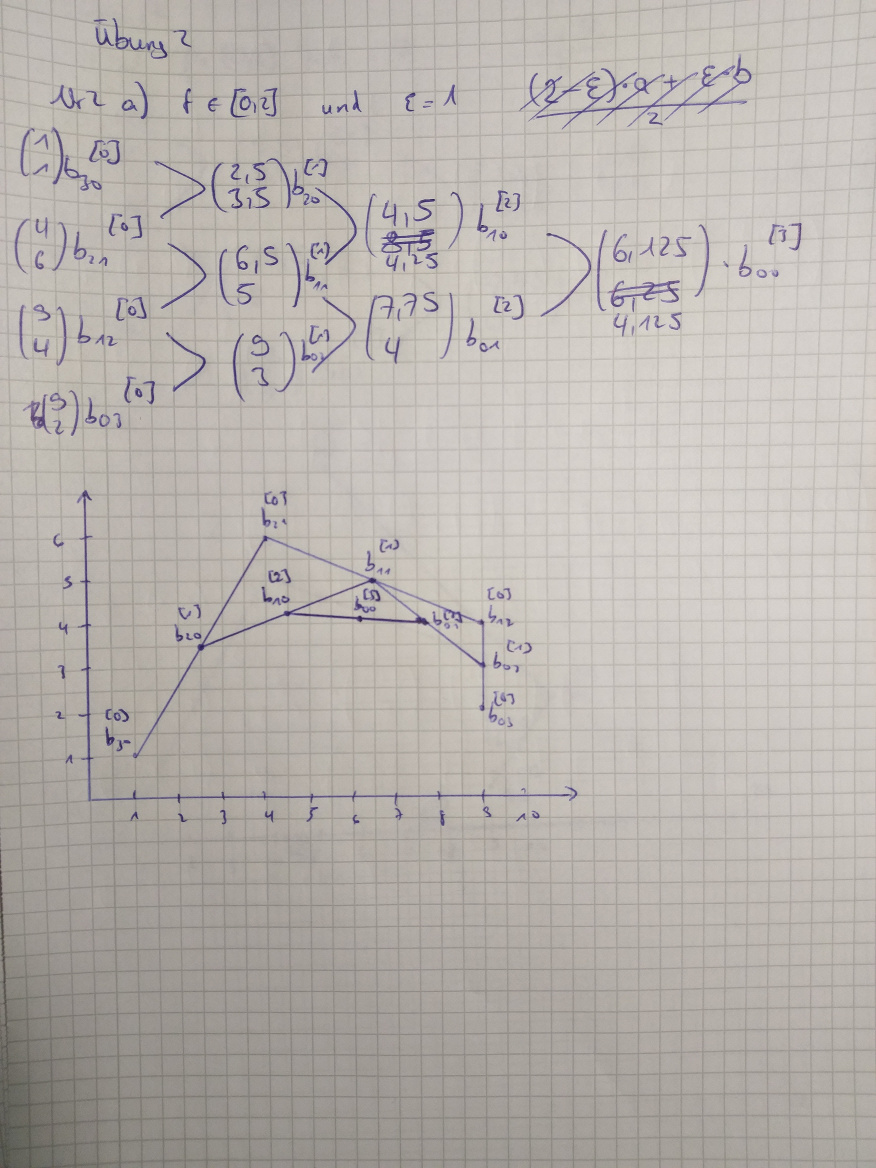
\includegraphics[width=\textwidth]{2a1}}
\end{center}
\begin{center}
  \makebox[\textwidth]{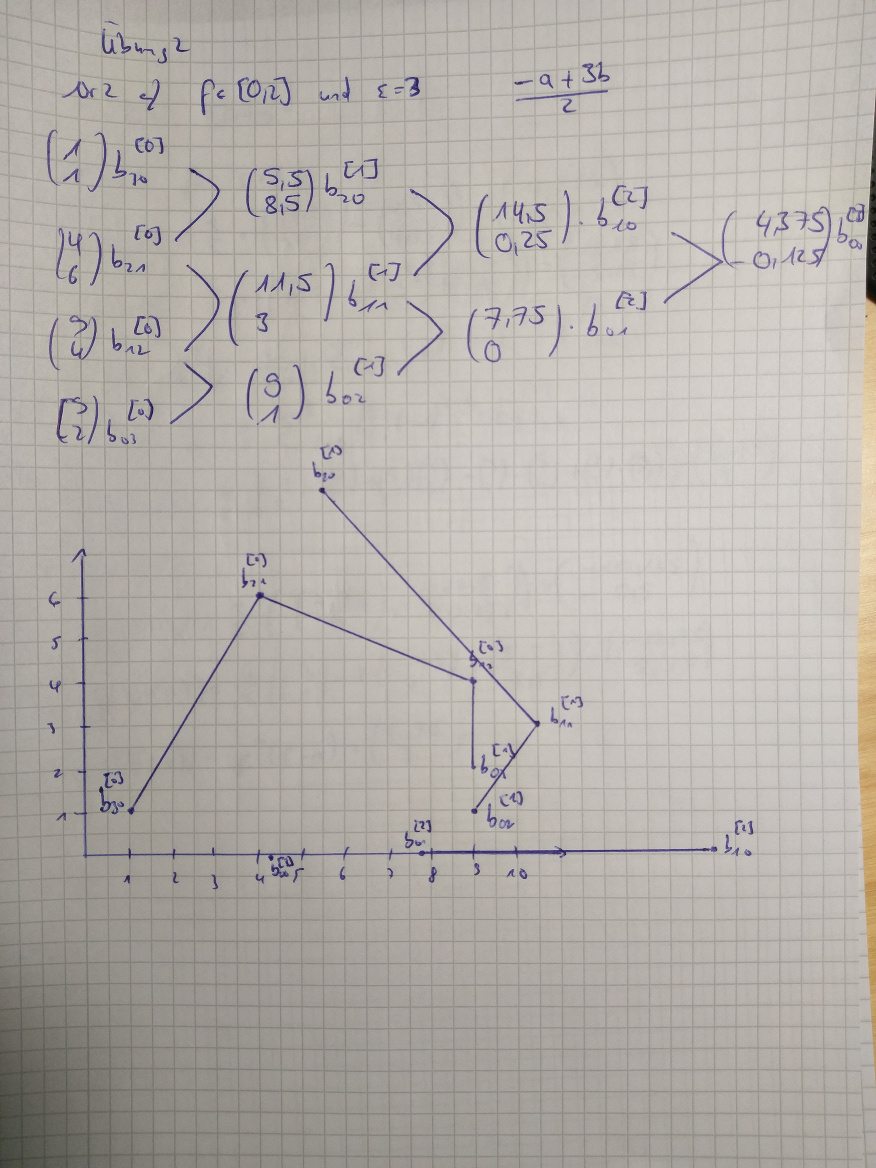
\includegraphics[width=\textwidth]{2a2}}
\end{center}
\subsubsection{1 Punkt}

\subsubsection{2 Punkte}
\begin{center}
  \makebox[\textwidth]{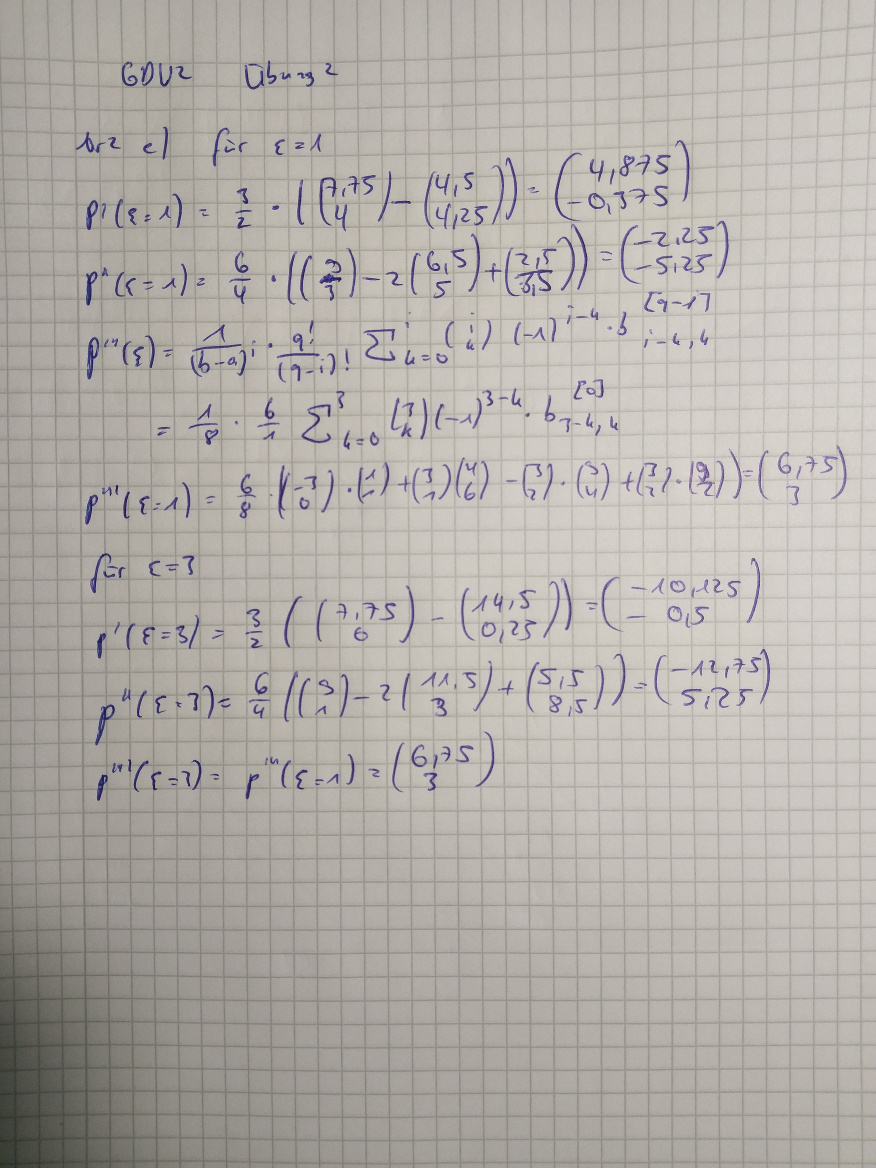
\includegraphics[width=\textwidth]{2c}}
\end{center}